\documentclass[a4paper,11pt]{article}

\usepackage{natbib,anysize,amsmath,amsopn,amssymb}
\marginsize{3cm}{3cm}{3cm}{3cm}

\renewcommand{\today}{\begingroup
\number \day\space  \ifcase \month \or January\or February\or March\or 
April\or May\or June\or July\or August\or September\or October\or 
November\or December\fi 
\space  \number \year \endgroup}

\renewcommand{\vec}[1]{\boldsymbol{#1}}
\newcommand{\gvec}[1]{\boldsymbol{#1}}
\newcommand{\mat}[1]{\mathbf{#1}}
\newcommand{\gmat}[1]{\boldsymbol{#1}}

\DeclareMathOperator{\E}{\boldsymbol{\mathbb{E}}}
\DeclareMathOperator{\Var}{Var}
\DeclareMathOperator{\Cov}{Cov}
\def\vecx{\vec{x}}
\def\vecy{\vec{y}}
\def\vecX{\vec{X}}
\def\vecY{\vec{Y}}

%%%%%%%%%%%%%%%%%%%%%%%%%%%%%%%%%%%%%%%%%%%%%%%%%%%%%%%%%%%%%%%%%%%%%%%%%
%%% Change this for a different vignette
%\VignetteIndexEntry{prim} 
%%%%%%%%%%%%%%%%%%%%%%%%%%%%%%%%%%%%%%%%%%%%%%%%%%%%%%%%%%%%%%%%%%%%%%%%%

\title{prim: an R package for Patient Rule Induction Method (PRIM) estimation of highest density difference regions}
\author{Tarn Duong \\ Department of Statistics, University of New South Wales \\ Sydney Australia}



%\SweaveOpts{}
\usepackage{/usr/lib/R/share/texmf/Sweave}
\begin{document}


\maketitle

\section{Introduction}

The Patient Rule Induction Method (PRIM) was introduced
by \citet*{friedman99}. It is a technique from data mining 
for finding `interesting' regions in high-dimensional data. 
We start with regression-type data $(\vecX_1, Y_1), \dots, (\vecX_n, Y_n)$
where $\vecX_i$ is $d$-dimensional and $Y_i$ is a scalar response variable.
We are interested in the conditional expectation function
$$
m(\vecx) = \E (Y | \vecx).    
$$
In the case where we have a single sample then PRIM
finds regions which correspond to the modal regions of $m(\vecx)$. 
These regions are closely related to the highest density regions (HDR) of 
\citet*{hyndman96}, defined in the form, for some threshold $\tau$,
$$
\lbrace m(\vecx) \geq \tau \rbrace.
$$
In the case where we have 2 samples, we can label the response as 
$$Y_i = \begin{cases} 1 & \mathrm{if} \ \vecX_i \ \mathrm{is \ from \ sample\ 1} \\
 -1 & \mathrm{if} \ \vecX_i \ \mathrm{is \ from \ sample\ 2.}
\end{cases}
$$
Then PRIM finds the regions where the samples are most different. 
Here we have a positive HDR (where sample 1 points dominate)
and a negative HDR (where sample 2 points dominate).

 


\section{Bivariate 1-sample PRIM}

We use a subset of the \texttt{Boston} 
data set in the \texttt{MASS} library. It contains
housing data measurements for 506 towns in the Boston, USA area.
For the explanatory variables, we
take the nitrogen oxides concentration in parts per 10 million (\texttt{nox}) 
and the average number of room per dwelling (\texttt{rm}). The 
response is the per capita crime rate (\texttt{crim}). 
We are interested in characterising those areas with higher crime rates
in order to provide better support infrastructure.

\begin{Schunk}
\begin{Sinput}
> library(prim)
> library(MASS)
> data(Boston)
> x <- Boston[, 5:6]
> y <- Boston[, 1]
> boston.prim <- prim.box(x = x, y = y, threshold.type = 1)
\end{Sinput}
\end{Schunk}
The default settings for \texttt{prim.box} are
\begin{itemize}
\item peeling quantile: \texttt{peel.alpha=0.05}
\item pasting is carried out: \texttt{pasting=TRUE} 
\item pasting quantile: \texttt{paste.alpha=0.01}
\item minimum box mass (proportion of points inside a box): 
 \texttt{mass.min=0.05} 
\item \texttt{threshold} is the overall mean of the response variable \texttt{y}
\item search for positive and negative HDR: \texttt{threshold.type=0}
\end{itemize}
We use the default settings except we wish to only find high crime areas 
$\lbrace m(\vecx) \geq \texttt{threshold} \rbrace$
so we set \texttt{threshold.type=1}. 

We view the output using a \texttt{summary} command. This displays three
columns: the box mean, the box mass, and the HDR indicator 
(1 = positive HDR, --1 = negative HDR). Each line is a summary
for each box, as well as an overall summary. Any box which is asterisked
indicates that it does not form part of the HDR estimate.
There is one box which contains 42.89\% of the towns
and where the average crime rate is 7.622. This is our HDR estimate. 
This regions comprises the bulk
of the high crime areas, and is described in terms of 
nitrogen oxides levels in $[0.5341, 0.7400]$ 
and average number of rooms in $[3.0391, 7.0691]$.
The other 57.11\% of the
towns have an average crime rate of 0.6036.

\begin{Schunk}
\begin{Sinput}
> summary(boston.prim)
\end{Sinput}
\begin{Soutput}
         box-mean  box-mass box-ind
box1    7.6222290 0.4288538       1
box2*   0.6035267 0.5711462      NA
overall 3.6135236 1.0000000      NA

* - box not in highest density region at level = 3.613524 

Box limits for box1
       nox     rm
min 0.5341 3.0391
max 0.7400 7.0691

Box limits for box2
        nox      rm
min 0.33640 3.03910
max 0.92446 9.35409
\end{Soutput}
\end{Schunk}

We plot the PRIM boxes, including 
all those towns whose crime rate exceeds 3.5. Thus 
verifying that the majority of high crime towns fall inside the
HDR.
\begin{Schunk}
\begin{Sinput}
> plot(boston.prim, col = "transparent")
> points(x[y > 3.5, ])
\end{Sinput}
\end{Schunk}
\setkeys{Gin}{width=0.45\textwidth}
\begin{center}
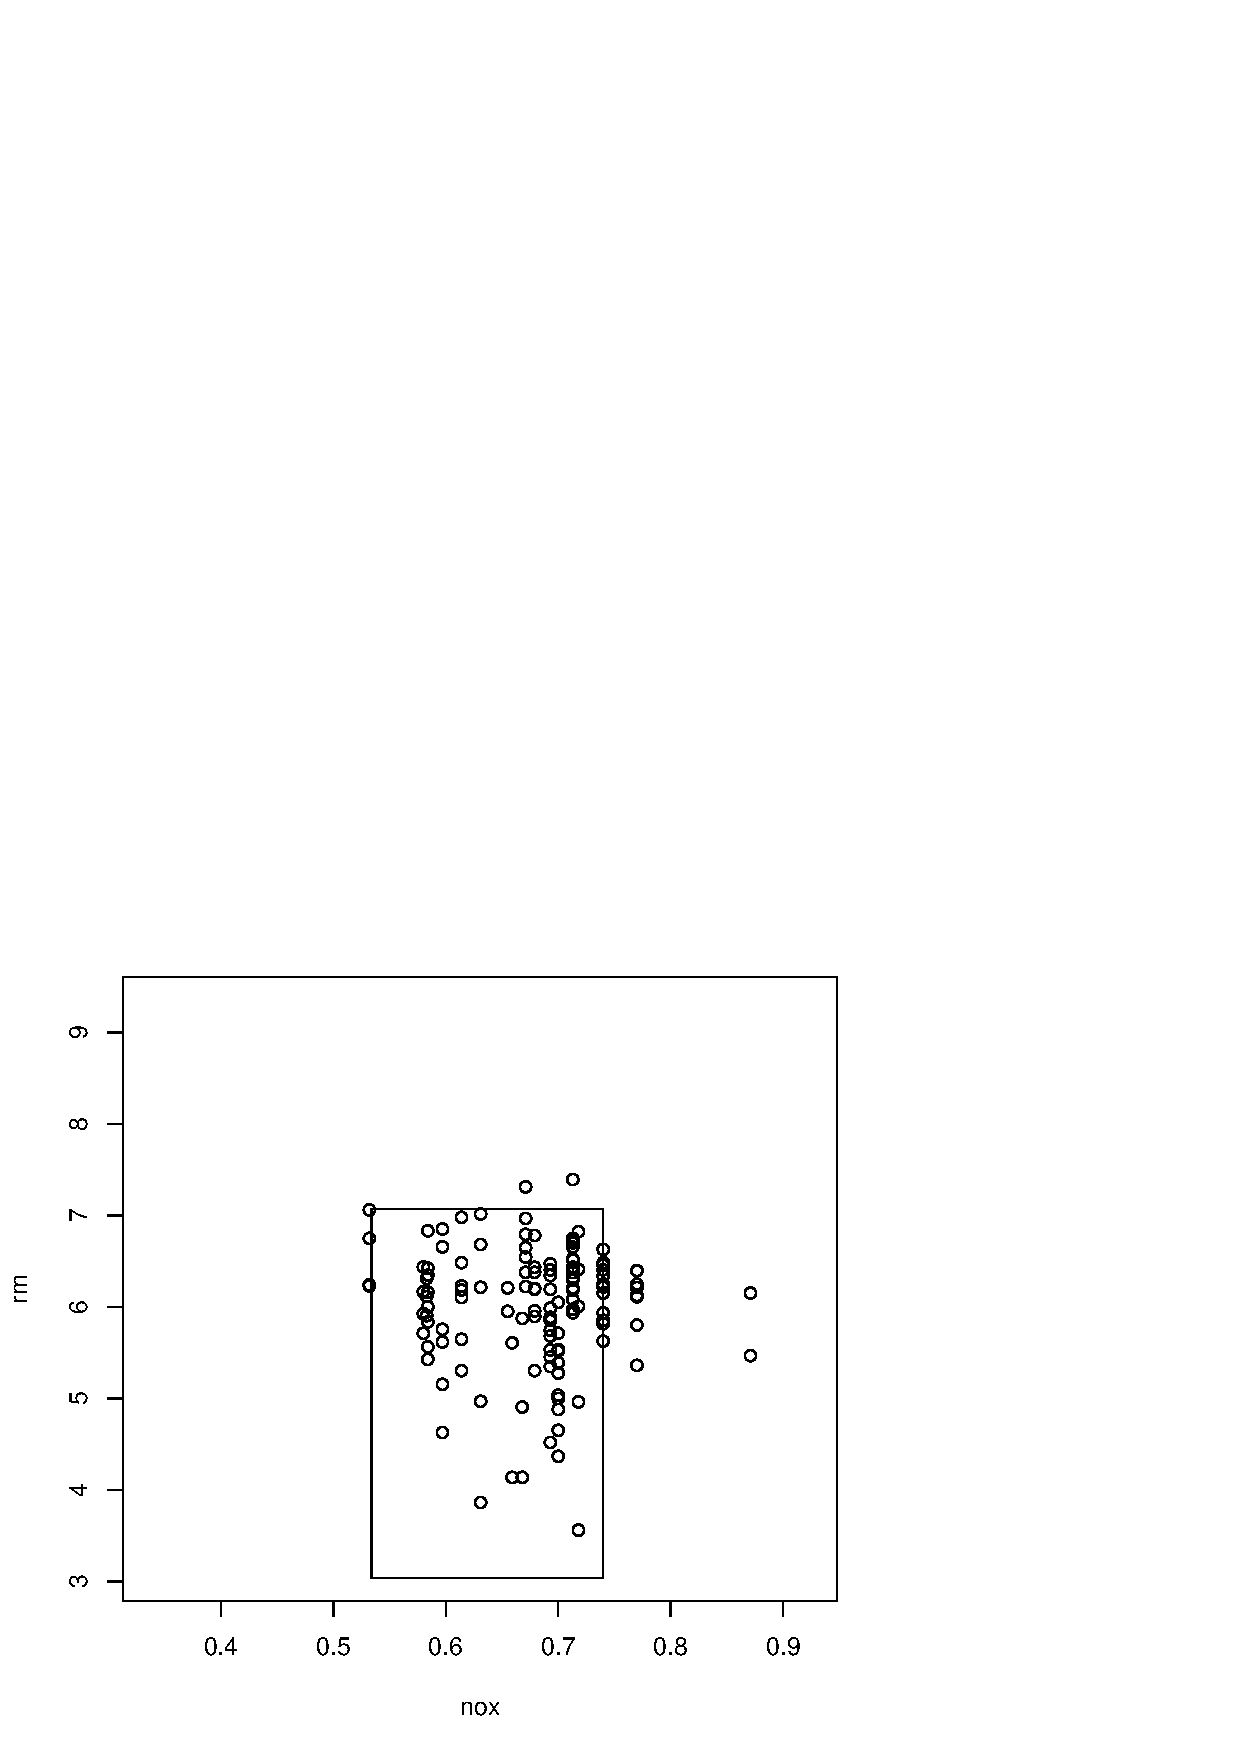
\includegraphics{prim-004}
\end{center}
There are many options for the graphical display. See
the help guide for more details \texttt{?plot.prim}.


\section{Quinti-variate highest density regions}
We started with a bivariate example since it is easy to visualise the
results. However, PRIM was developed with much higher dimensional data in
mind. So we look at a 5-dimensional data set (\texttt{quasiflow}) included in the
\texttt{prim} library. It is a randomly generated data set from 
two normal mixture distributions whose structure mimics  
some light scattering data, taken from a machine known as a flow cytometer. 
 
\begin{Schunk}
\begin{Sinput}
> library(prim)
> data(quasiflow)
> yflow <- quasiflow[, 6]
> xflowp <- quasiflow[yflow == 1, 1:5]
> xflowm <- quasiflow[yflow == -1, 1:5]
> xflow <- rbind(xflowp, xflowm)
\end{Sinput}
\end{Schunk}
We can think of \texttt{xflowp} as flow cytometric measurements from an
HIV+ patient, and \texttt{xflowm} from an HIV-- patient.
\begin{Schunk}
\begin{Sinput}
> xlim <- c(-30, 550)
> ylim <- c(-30, 550)
> pairs(xflowp[1:100, ], xlim = xlim, ylim = ylim)
> pairs(xflowm[1:100, ], xlim = xlim, ylim = ylim)
\end{Sinput}
\end{Schunk}

\setkeys{Gin}{width=0.45\textwidth}
\begin{center}
\begin{tabular}{cc}
HIV+ & HIV-- \\
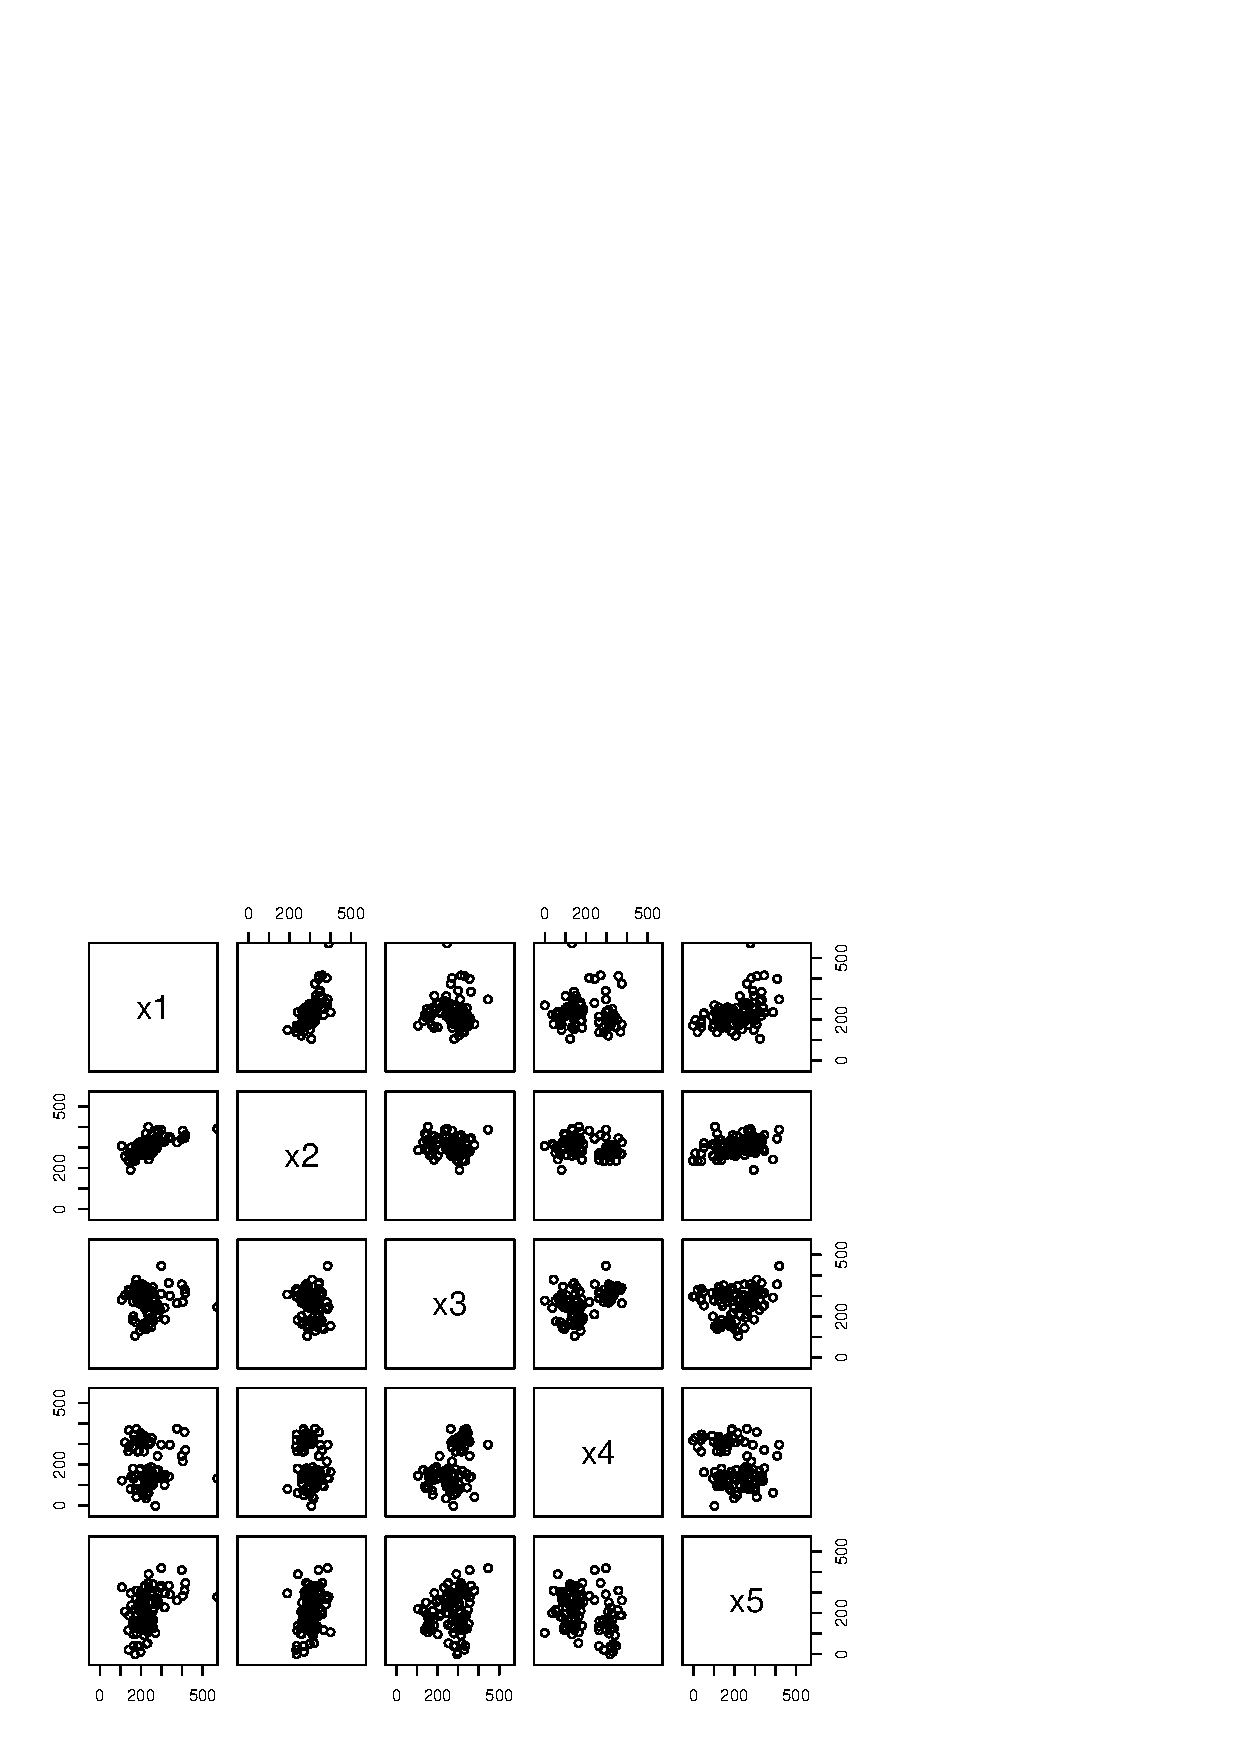
\includegraphics{prim-007}
&
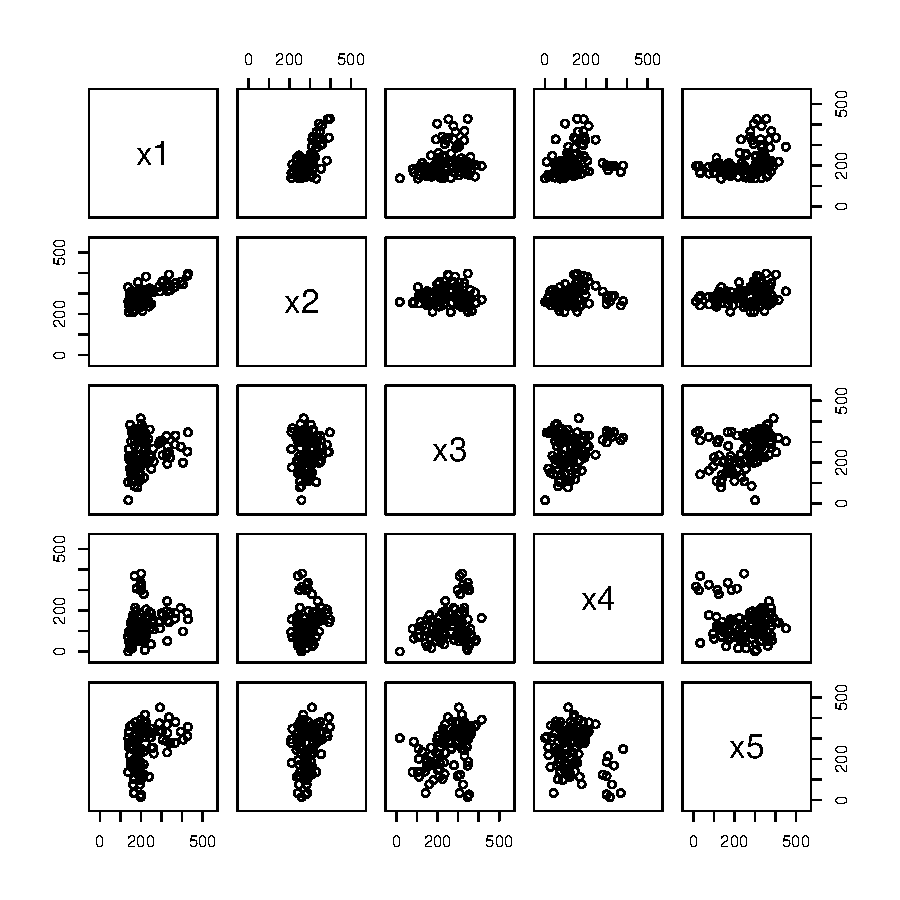
\includegraphics{prim-008}
\end{tabular}
\end{center}

There are two ways of using \texttt{prim.box} to estimate where the 
two samples are most different (or equivalently 
to estimate the HDRs of the difference of the density functions). 
In the first way, we assume that we have suitable
values for the thresholds. Then we can use
\begin{Schunk}
\begin{Sinput}
> qflow.thr <- c(0.85, -0.6)
> qflow.prim <- prim.box(x = xflow, y = yflow, threshold = qflow.thr, 
+     threshold.type = 0)
\end{Sinput}
\end{Schunk}

An alternative is compute PRIM box sequences which cover the entire data range, 
and then use \texttt{prim.hdr} to experiment with different threshold values.
This two-step process is more efficient and faster than calling \texttt{prim.box}
for each different threshold.
We're happy with the positive HDR threshold so we can compute the positive
HDR directly: 
\begin{Schunk}
\begin{Sinput}
> qflow.hdr.plus <- prim.box(x = xflow, y = yflow, threshold = 0.85, 
+     threshold.type = 1)
\end{Sinput}
\end{Schunk}
On the other hand, we're not sure about the negative HDR thresholds.
\begin{Schunk}
\begin{Sinput}
> qflow.minus <- prim.box(x = xflow, y = yflow, threshold.type = -1)
> qflow.hdr.minus1 <- prim.hdr(qflow.minus, threshold = -0.3, threshold.type = -1)
> qflow.hdr.minus2 <- prim.hdr(qflow.minus, threshold = -0.4, threshold.type = -1)
> qflow.hdr.minus3 <- prim.hdr(qflow.minus, threshold = -0.6, threshold.type = -1)
\end{Sinput}
\end{Schunk}
After examining the summaries and plots, we  
choose \texttt{qflow.hdr.minus3} to combine with \texttt{qflow.hdr.plus}.
\begin{Schunk}
\begin{Sinput}
> qflow.prim2 <- prim.combine(qflow.hdr.plus, qflow.hdr.minus3)
\end{Sinput}
\end{Schunk}
In the plot below, the positive HDR is coloured orange, and the 
negative HDR is coloured blue.  
These 5-dimensional HDRs can be more or less distinct some 2-dimensional
projections e.g. $(x_3, x_4)$ whereas in others they
can overlap considerably e.g. $(x_1, x_2)$.
We conclude that there are more HIV+ patients
within the orange regions and more HIV-- patients within the blue regions. 
(The plot is not exactly what is produced by the \texttt{plot} command
below -- the number of data points has been thinned for purposes of clarity).
 
\begin{Schunk}
\begin{Sinput}
> xmin <- rep(-30, 5)
> xmax <- rep(550, 5)
> col <- qflow.prim2$ind
> col[col == 1] <- "orange"
> col[col == -1] <- "blue"
> plot(qflow.prim2, col = col, xmin = xmin, xmax = xmax)
\end{Sinput}
\end{Schunk}

\setkeys{Gin}{width=0.65\textwidth}
\begin{center}
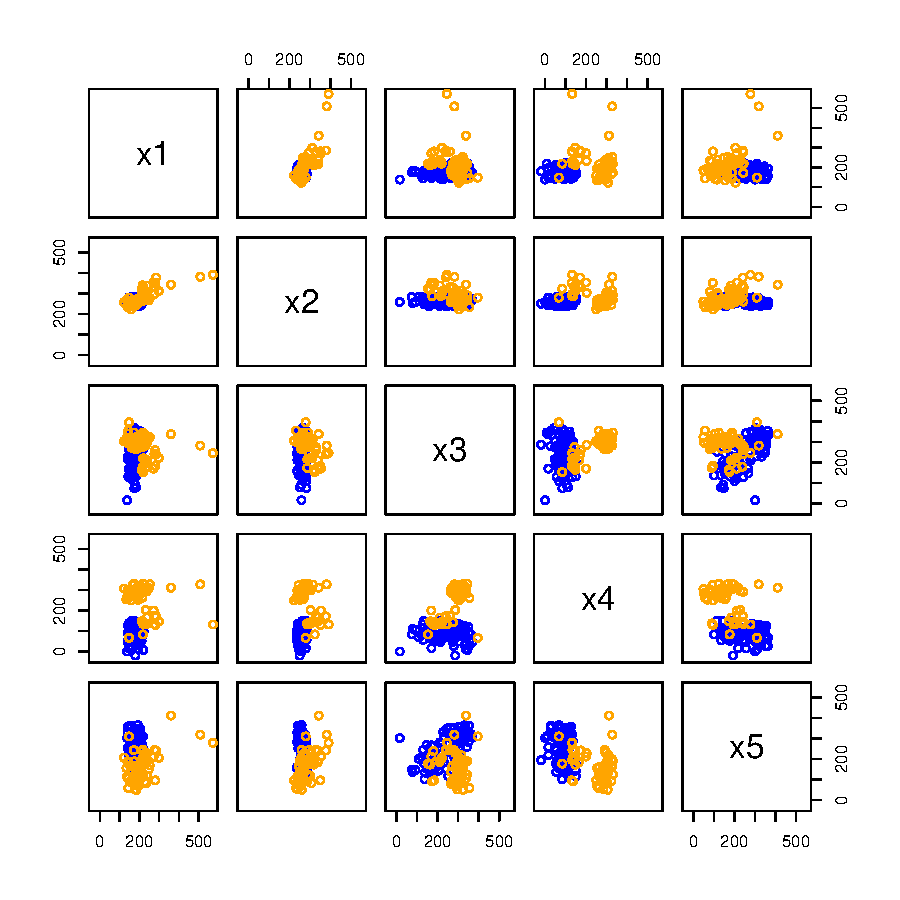
\includegraphics{prim-014}
\end{center}

The next step is to study the statistical properties of these HDR estimates.
For some preliminary work, see \cite*{duong07b}.

\bibliographystyle{apalike}


\begin{thebibliography}{}

\bibitem[{Duong, Koch and Wand}, 2007]{duong07b}
Duong, T., Koch, I., and Wand, M.~P. (2007).
\newblock A generalised chi-squared test for comparing samples from data rich
  sources: an example from flow cytometry.
\newblock In preparation.

\bibitem[Friedman and Fisher, 1999]{friedman99}
Friedman, J.~H. and Fisher, N.~I. (1999).
\newblock Bump-hunting for high dimensional data.
\newblock {\em Statistics and Computing}, \textbf{9}, 123--143.

\bibitem[Hyndman, 1996]{hyndman96}
Hyndman, R.~J. (1996).
\newblock Computing and graphing highest density regions.
\newblock {\em The American Statistician}, \textbf{50}, 120--126.

\end{thebibliography}

%\bibliography{/c/tduong/home/research/references}

\end{document}
